\documentclass[conference]{IEEEtran}

\usepackage{graphicx}
\usepackage{amsmath}
\usepackage{amsfonts}
\usepackage{cite}
\usepackage{listings}
\usepackage{xcolor}
\usepackage{caption}
\usepackage{array}

\lstset{
    basicstyle=\ttfamily\footnotesize,
    keywordstyle=\bfseries\color{blue},
    commentstyle=\itshape\color{green},
    stringstyle=\color{red},
    breaklines=true,
    captionpos=b,
    numbers=left,
    numberstyle=\tiny\color{gray},
    frame=single,
    backgroundcolor=\color{lightgray!20},
    tabsize=4
}

\title{Simulations of Hexadecimal Counters via the 74LS161 Integrated Circuit -- Applications of Visual-Based Multisim and Verilog Projections}

\author{
    \IEEEauthorblockN{Xiangbo Cai\IEEEauthorrefmark{1}, Peter Pena\IEEEauthorrefmark{2}}
    \IEEEauthorblockA{\IEEEauthorrefmark{1}Department of Electrical \& Computer Engineering, Michigan State University, East Lansing, MI 48825, USA}
    \IEEEauthorblockA{\IEEEauthorrefmark{2}Department of Computer Science \& Engineering, Michigan State University, East Lansing, MI 48825, USA}
}

\begin{document}

\maketitle

\begin{abstract}
This project focuses on exploring the characteristics of the 74LS161 integrated circuit (IC) in a more specific set tailored for visual simulation. The exploration extends beyond theoretical analysis, incorporating practical experiments and simulations that highlight the IC's real-world features. Specifically, the project delves into timing analysis and the impact of load variations on the 74LS161's performance, which are crucial for understanding its operation in complex circuits. The article primarily discusses the principles of the 74LS161 IC digital logic, relevant features, and then applies the 74LS161 to a hexadecimal counter followed by simulations. The simulations are divided into two types: the first using NI Multisim software to generate circuit diagrams and perform static simulations, and the second involving code in Vivado Verilog to generate dynamic waveforms for simulation. The visual results of these two simulation methods are compared and evaluated against the actual properties and minor applications of the 74LS161 IC.
\end{abstract}

\begin{IEEEkeywords}
74LS161, Integrated Circuit, Simulation, Hexadecimal Counter, NI Multisim, Vivado Verilog
\end{IEEEkeywords}

\section{Introduction}
In everyday life, the increasingly popular need for higher efficacy chip characteristics drives innovation in digital circuitry, particularly in the realm of counters. This article aims to comprehensively explore the practical applications \cite{Long2024} and operational intricacies of a crucial component within this domain. The 74LS161 counter chip, especially in the realm of counters, is a vitally relevant chip in digital circuits.

It introduces the method of analyzing the operations of the 74LS161 IC with certain inputs and representing the static and physical manifestation of these operations with simulation software like NI Multisim. Additionally, the logic analyzer in Multisim, which can intuitively describe the working process of the counter, can display various input and status output signals of the counter in both a synchronous and multi-track manner \cite{Li2021}.

Furthermore, the usage of Vivado’s Verilog modeling software to simulate the underlying circuit logic of the 74LS161 chip allows for a clearer model in the electronic efficacy of a more dynamic implementation. By assigning a testbench to test the corresponding output results and simulate the waveforms, comparison of the simulated waveforms and logical outputs generate visuals which verify increased efficacy in the implementation of hexadecimal counters \cite{Yashas2019}.

Overall, in testing certain features of the 74LS161 chip by providing more refined visuals of practical implications of enhanced chip characteristics, this article aims to contribute to the advancement of digital circuit design and visualization. Its applications in alternative counting such as the hexadecimal system are vital to creating more accurate simulations and ultimately more practical and efficient electrical systems \cite{Zhang2016}.

\section{Counter Logic \& Features}

\subsection{Introductory Logic regarding counter}
According to binary addition principles \cite{Reitwiesner1960}, when adding 1 to a multi-digit binary number, if all the bits below the i-th bit are 1 (from i-1, i-2, …, 1), then the i-th bit will change state (from 0 to 1 or from 1 to 0). The state of the lowest bit changes every time 1 is added. The following diagram shows a state:

\begin{figure}[h]
    \centering
    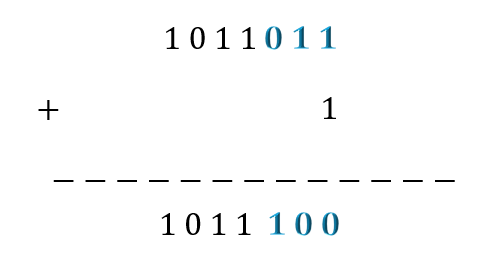
\includegraphics[width=0.3\textwidth]{binary_counter}
    \caption{Example of binary addition}
\end{figure}

Synchronous counters are typically constructed using "T flip-flops" \cite{Irving1976} with two main structural forms. One form controls the state of the T input terminal. When each CLK signal (counting pulse) arrives, the flip-flops whose inputs at the control terminal $T_i$ should be flipped are set to $T_i=1$, while those that shouldn't be flipped are set $T_i=0$. The other form controls the clock signal; when each counting pulse arrives, it is only applied to the CLK input terminals of the flip-flops that should be flipped while those that shouldn't be flipped remain unchanged. At the same time, all flip-flops are set to $T=1$. Therefore, the different states of the counter circuit can be used to record the number of inputs CLK pulses.

Furthermore, when controlling through the T terminal's state, the logic expression for the input terminal of the i-th flip-flop should be:

\begin{equation}
    T_i = Q_{i-1} Q_{i-2} … Q_1 Q_0 = \prod_{j=0}^{i-1} Q_j \quad (i=1, 2, …, n-1)
\end{equation}

\subsection{Background Information with the 74LS161 setup}
The 74LS161 is a synchronous 4-bit counter IC (Integrated Circuit) from the 74LS family of TTL (Transistor-Transistor Logic) chips \cite{Jung2003}. It is designed to count up or down in binary increments depending on the logic levels applied to its control inputs. 74LS161 can reach, through input tweaks, the functionality of a 4-bit hexadecimal counter.

\begin{table}[h]
    \centering
    \caption{Project's "tweaked" input and output types of the 74LS161 chip}
\begin{tabular}{|>{\centering\arraybackslash}m{0.75cm}|>{\centering\arraybackslash}m{3cm}|>{\centering\arraybackslash}m{1cm}|>{\centering\arraybackslash}m{2.5cm}|}
\hline
\textbf{Input} & \textbf{Description} & \textbf{Output} & \textbf{Description} \\ \hline 
clk & time clock, period happen & tc & carry out value \\ 
clr & clear value, reset to all 0 & Q[3:0] & count output number \\ 
ld & enable to load number &  &  \\ 
EP & work control 1 &  &  \\ 
ET & work control 2 &  &  \\ 
P[3:0] & user input initial value &  &  \\ \hline
\end{tabular}
\end{table}

In practical production of counter chips, additional control circuits are often added to increase the circuit's flexibility. The designed circuit should not only have the function of a binary adder counter but also have additional functions such as "preset number," "hold," and "asynchronous clear." In the diagram, "ld" is the preset control terminal, "P[3:0]" is the input terminal, and "EP" and "ET" are the operating state control terminals. The table below shows the functions associated for this project in a given 4-bit 74LS161.

\begin{table}[h]
    \centering
    \caption{Functions for the representation of the 4-bit synchronous hexadecimal 74LS161}
    \begin{tabular}{|c|c|c|c|c|c|c|}
    \hline
    \textbf{clk} & \textbf{clr} & \textbf{ld} & \textbf{EP} & \textbf{ET} & \textbf{Output State} \\ \hline
    \texttimes & 0 & \texttimes & \texttimes & \texttimes & Set to 0000 \\ 
    $\uparrow$ & 1 & 0 & \texttimes & \texttimes & Set to input \\ 
    \texttimes & 1 & 1 & 0 & 1 & Not changed \\ 
    \texttimes & 1 & 1 & \texttimes & 0 & NC but tc=0 \\ 
    $\uparrow$ & 1 & 1 & 1 & 1 & Counts \\ \hline
    \end{tabular}
\end{table}

\section{Simulation of 74LS161 on NI Multisim}

Utilizing the preset logic bases discussed, the simulation of the 74LS161 integrated circuit can be applied by using counting-base types, like hexadecimal, physically. “In many applications, [these] counters can be designed using these available ICs. In case any other sequence of count or modules is required, then the circuit can be designed. These methods are validated through experiments and, if correct, in practice can be used directly” \cite{Zhao2011}. By summarizing the tables created, the resulting "pseudocode" can be used to easily create NI Multisim diagrams.

When clr=0, "asynchronous clear" occurs. When clr=1 and ld=0, synchronous load occurs. When clr=ld=1, and EP=ET=1, the 74LS161 exhibits addition counting that is performed in binary two's complement. When clr=ld=1, and EP*ET=0, the counting state remains unchanged. Sequentially, it is natural that the generation of the Multisim logic to simulate the above result should further expose the desired efficacy increase expectations.

As can be seen from Figure 2, the S2 is linked with the clr, and s1 is linked with the ld. Via a Multisim circuit model, the types clr=0 and ld=0, and our output=0 are set. In Figure 3, the types clr=1 but ld=1 are set so that the output vector Q loads the input vector P, and, as the initial input vector P in the graph is set to be 6, the output should be 6.

\begin{figure}[h]
    \centering
    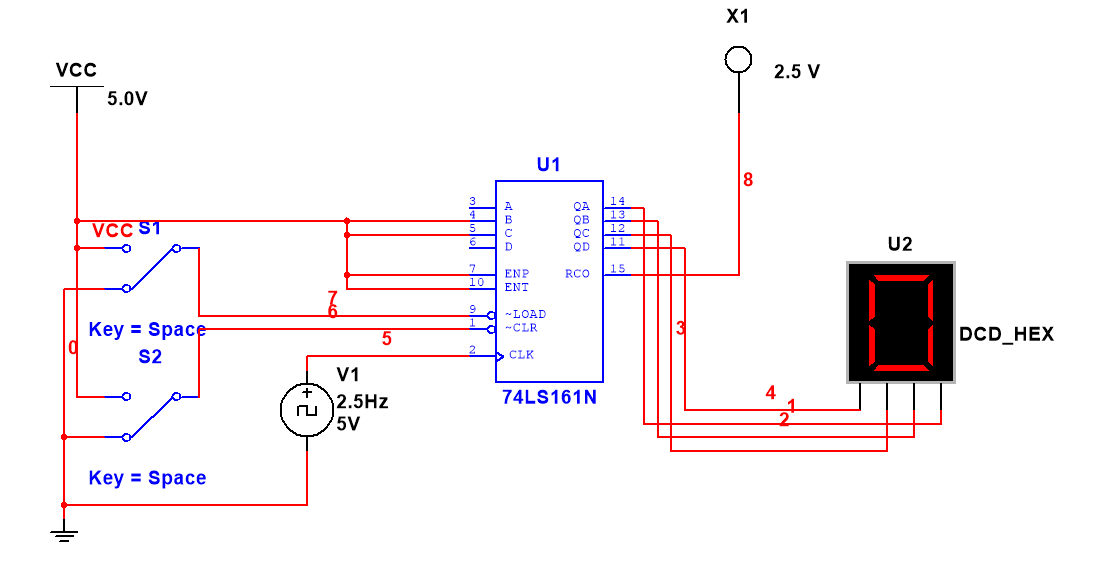
\includegraphics[width=0.5\textwidth]{multisim_clr_ld_0}
    \caption{When clr=ld=0, the output is set to 0}
\end{figure}

\begin{figure}[h]
    \centering
    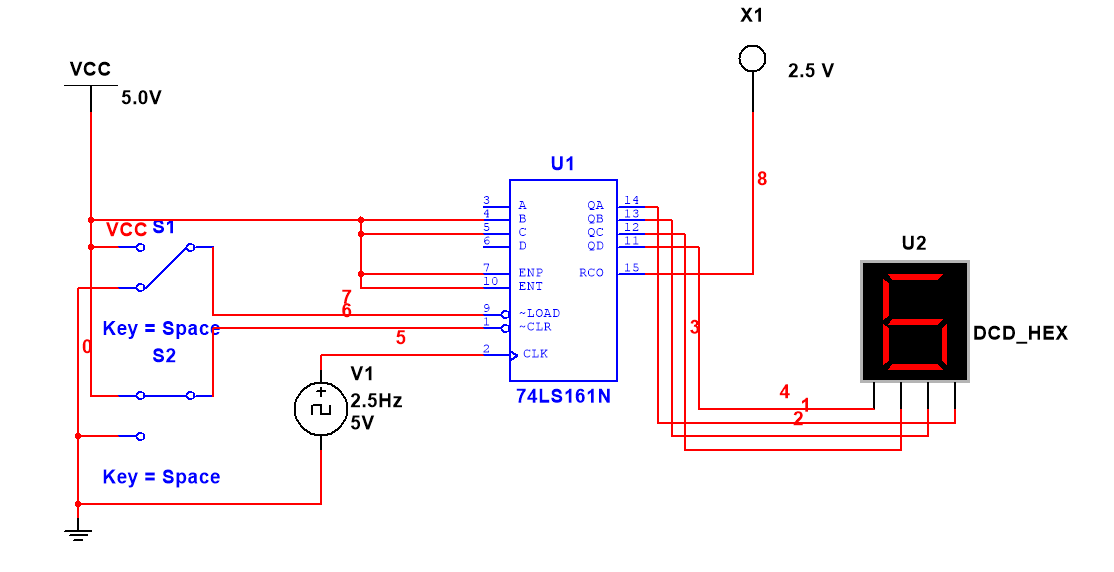
\includegraphics[width=0.5\textwidth]{multisim_clr_1_ld_0}
    \caption{When clr=1 but ld=0, the output Q loads the input vector P, set to 6}
\end{figure}

When EP and ET are also set to 1, the 74LS161 will start to count. The static figure for the moment when the output result increments to 8 during the second cycle is captured below.

\begin{figure}[h]
    \centering
    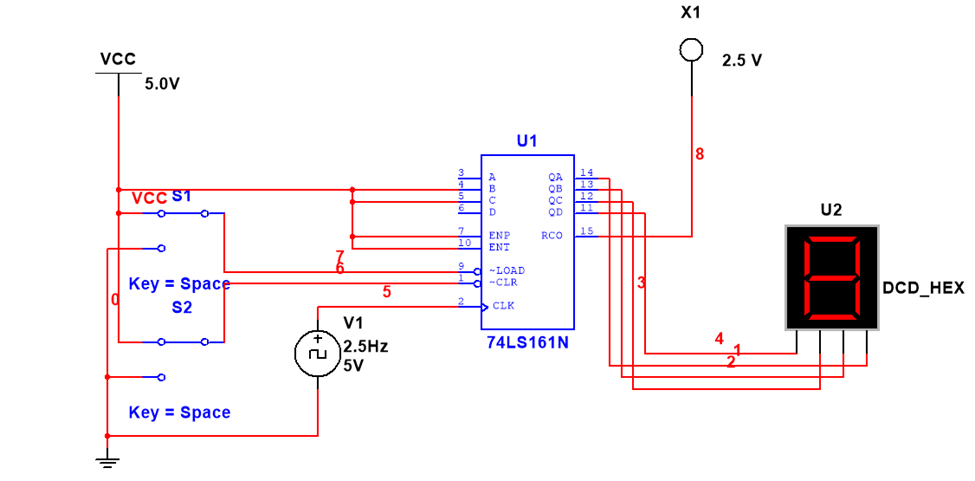
\includegraphics[width=0.45\textwidth,height=0.175\textheight]{multisim_count_8}
    \caption{When clk=ld=1 and ET=EP=1, output starts to count}
\end{figure}

When the output result reaches F (16 in decimal), the carry output TC will flicker indicating that the part is about to carry once. The output P [3:0] will then return to 0 and continue counting while TC will flicker for an extremely short period (becoming 1) and then it will extinguish (becoming 0) again.

\begin{figure}[h]
    \centering
    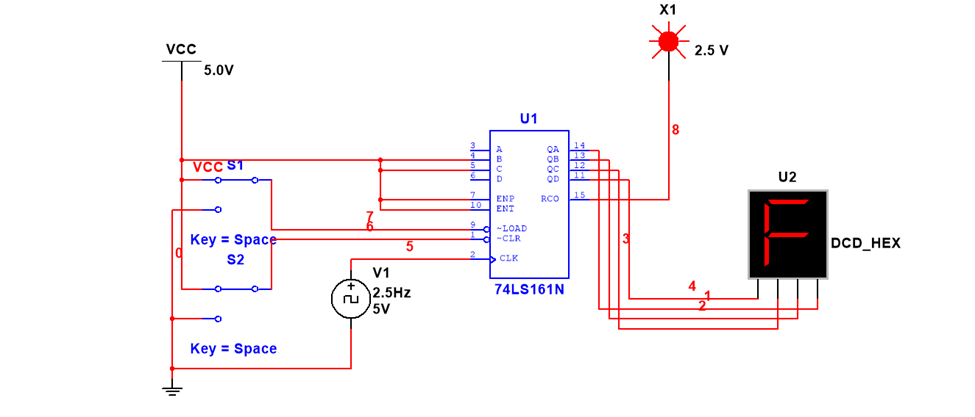
\includegraphics[width=0.5\textwidth]{multisim_count_f}
    \caption{When clr = ld = 1 and EP=ET=1 and Q reach highest F(16) tc flips to 1}
\end{figure}

\section{Simulation of 74LS161 on Verilog Code}
The underlying logic of the 74LS161 chip can be accurately transformed into corresponding Vivado Verilog code for implanted simulation. In the module design, we include input ports clk, clr, ld, an input vector p [3:0], output ports tc, a carry-out display bit, and output vector q [3:0]. Based on the logic summary of the 74LS161 chip in the second part as well as a basic understanding of Verilog basic systems for coding, the corresponding circuit code can be designed as follows. In the following Verilog code, `cet` can be used to represent the ET and `cep` for EP. As an alternative to the standard, the type `clr` is set as high active instead of negative active.

\begin{figure}[h]
    \centering
    \begin{lstlisting}[
        language=Verilog,
        caption={Verilog Code Design of the 74LS161 Module},
        xleftmargin=1cm,
        xrightmargin=1cm
    ]
module ttl_74161(
    input ld,
    input [3:0] p,
    output reg [3:0] q,
    input cet,
    input cep,
    input clk,
    output tc,
    input clr
 );
assign tc = cet & (&q);
initial begin
    q <= 0;
end
always @ (posedge clk or negedge clr) begin
    if (clr) begin
        q <= 0;
    end else begin
        if (ld == 1) begin
            q <= p; end
        if (cep & cet) begin
            q <= q + 1;
        end  
    end   
end
endmodule
    \end{lstlisting}
\end{figure}


According to the output results, three groups of test data can be set up—corresponding to the clear, load, and counting states respectively. The following is the related testbench code.

\begin{figure}[h]
    \centering
    \begin{lstlisting}[
        language=Verilog,
        caption={Verilog Code for the 74LS161 Testbench},
        xleftmargin=1cm,
        xrightmargin=1cm
    ]      
module ttl_74161_tb;

    // Inputs
    reg ld, cet, cep, clk, clr;
    reg [3:0] p;

    // Outputs
    wire [3:0] q;
    wire tc;

    // Instantiate the module under test
    ttl_74161 uut (
        .ld(ld),
        .p(p),
        .q(q),
        .cet(cet),
        .cep(cep),
        .clk(clk),
        .tc(tc),
        .clr(clr)
    );

    // Clock generation
    always begin
        #5 clk = ~clk;
    end
    // Reset
    initial begin
        ld = 0;
        p = 4'b0000;
        clk = 0;
        clr = 0;
        cep = 0;
        cet = 0;
    end
    
    // Test scenarios
    initial begin
        // Scenario 1: clr = 0
        #15 clr = 1;
        #15 clr = 0;
        #15 p = 3;
        // Scenario 2: clr = 1, ld = 1
        #15 ld = 1;

        // Scenario 3: clr = 1, ld = 1, cep = 1, cet = 1
        # 15 cep = 1; cet = 1;

        // End simulation
        #350 $finish;
    end
endmodule
    \end{lstlisting}
\end{figure}

Now using the code above, the result can be used to create visual signal simulations, also known as waveforms: Figure \ref{fig:initial_state} depicts the initial state where clr is set to 1, causing the output q [3:0] to be 0000 in binary as indicated by the `4b` prefix. This state is clearly highlighted by the pink line and the light bar in the accompanying photo, emphasizing the clarity of the representation. The simulation visual provides a visual confirmation of the expected behavior.

\begin{figure}[h]
    \centering
    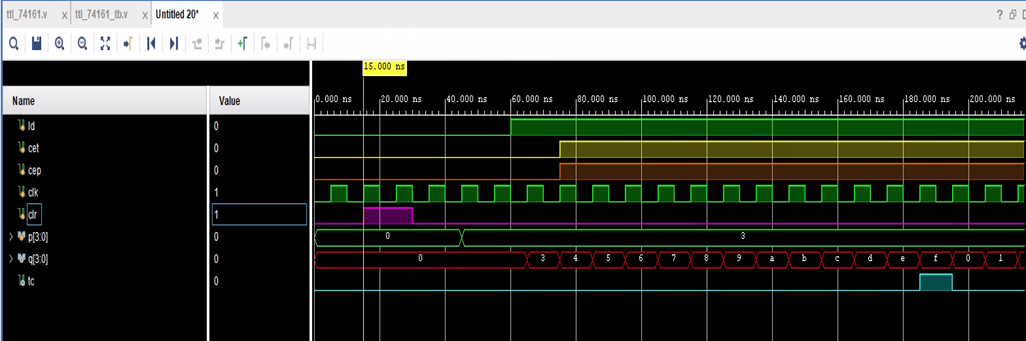
\includegraphics[width=0.5\textwidth]{verilog_simulation_1}
    \caption{When clr=1 all value is set to be zero}
    \label{fig:initial_state}
\end{figure}

Figure \ref{fig:load_value} shows the load value when active high (equal to 1) causes the input value p [3:0] to be loaded into q [3:0]. This behavior is clearly observable in the highlighted red vector and light bar section of the diagram. As depicted when the clock signal (clk) experiences a positive edge, the red vector begins to store the input p [3:0] vector value.

\begin{figure}[h]
    \centering
    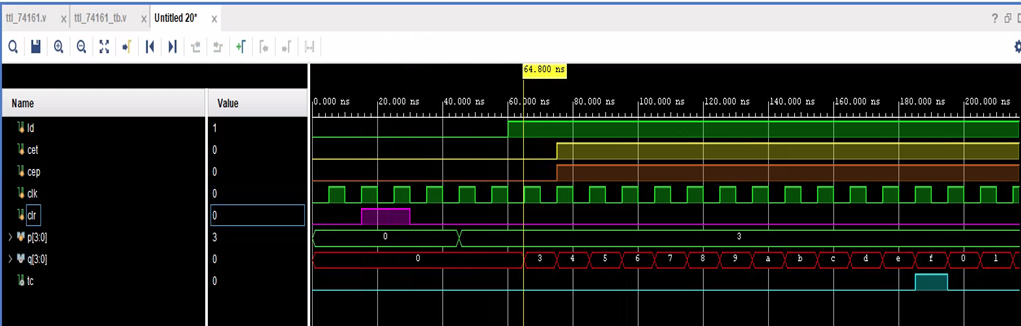
\includegraphics[width=0.5\textwidth]{verilog_simulation_2}
    \caption{When ld=1 the input p value 3 is loaded into output q [3:0]}
    \label{fig:load_value}
\end{figure}

In Figure \ref{fig:count_up} activating both control inputs cet and cep to 1 initiates the count-up sequence of the output value q [3:0] in hexadecimal. This behavior is clearly demonstrated in the diagram, indicating that when cet and cep are both high, the counting operation begins.

\begin{figure}[h]
    \centering
    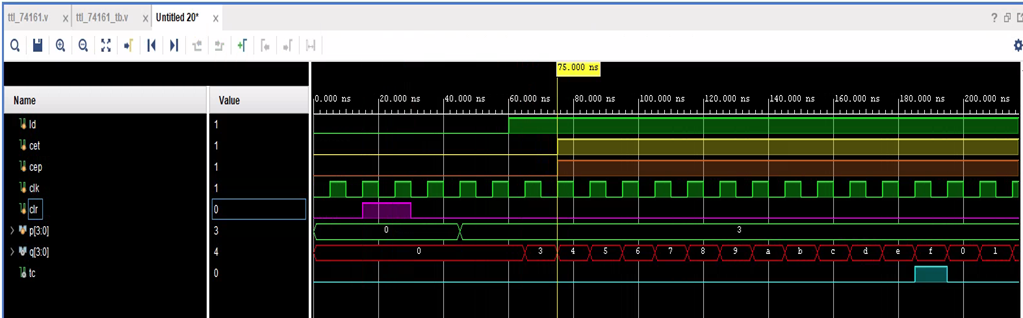
\includegraphics[width=0.5\textwidth]{verilog_simulation_3}
    \caption{When cet(ET)=cep(EP)=1 output q start to count up}
    \label{fig:count_up}
\end{figure}

When the output vector q [3:0] reaches `4b’1111`, we set the terminal count wrap (tc) to be 1 and q [3:0] will reset to `4b’0000` and restart, and tc back to 0. As can be seen in Figure \ref{fig:wrap_around}, the blue bar indicates the tc output situation.

\begin{figure}[h]
    \centering
    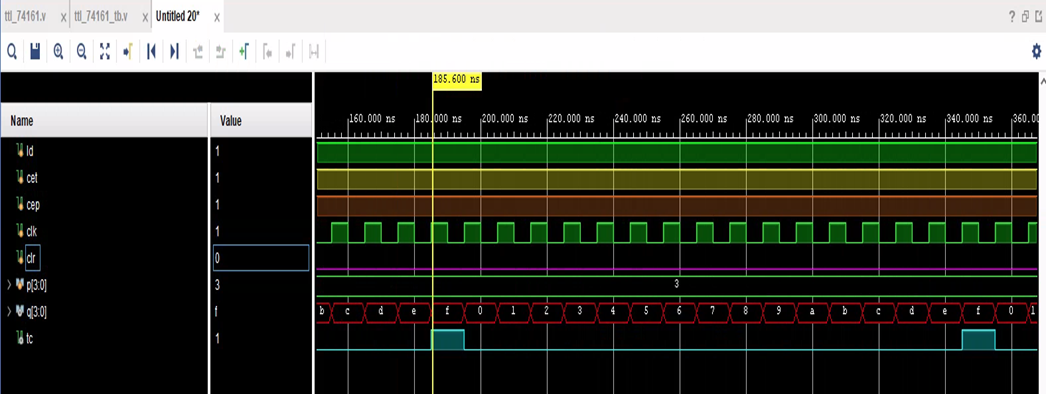
\includegraphics[width=0.5\textwidth, height=0.1\textheight]{verilog_simulation_4}
    \caption{Output vector q=4b'1111, tc flips to 1 and carry in}
    \label{fig:wrap_around}
\end{figure}

\section{Conclusion}
Utilizing these simulations shows the inherent workings of basic counting circuits, specifically 74LS161 IC, to show vulnerabilities and possible efficiencies in systems integrating them. By examining the logic of the 74LS161, the real model of the 74LS161 is transformed into a fully-fledged digital circuit model at the macro level. Simultaneously, for the underlying logic of the 74LS161, conversion of the chip results in Verilog code that relevantly embodies the logic through color-based visuals and highlights of circuit states in a dynamic setting. Compilation of this Verilog code simulated alongside the Multisim models produce the desired waveforms: clearly demonstrating increased time response in areas based on hexadecimal or more complex counting-based systems.

Further relating to the modern world through various digital logic applications and electronic devices, the applications of 74LS161 are very extensive \cite{Bao2021}. Counters, steppers, frequency dividers, pulse sequence generators, and automatic control systems can all be made more efficient and practical. The use of these circuits is becoming increasingly common and continues to benefit the progression of electronic-counter-system technology. Understanding how to better implement these circuits like 74LS161, especially through the use of simulation technology \cite{Deng2012}, is essential for us to have a deeper understanding of digital circuits and improve our increasingly digital world.

\bibliographystyle{IEEEtran}
\begin{thebibliography}{1}

\bibitem{Long2024}
Z. Long, “N-system counter design based on 74LS16X,” Ninth International Symposium on Sensors, Mechatronics, and Automation System (ISSMAS 2023), Mar. 2024. doi:10.1117/12.3014793

\bibitem{Li2021}
L. Li, L. Meng, and F. Wang, “Design and simulation of frequency divider circuit based on multisim,” \textit{E3S Web of Conferences}, vol. 268, p. 01058, 2021. doi:10.1051/e3sconf/202126801058

\bibitem{Yashas2019}
D. Yashas, P. S. Hari Babu, and N. Shylashree, “UVM-based logic verification of input output interface,” 2019 4th International Conference on Recent Trends on Electronics, Information, Communication \& Technology (RTEICT), May 2019. doi:10.1109/rteict46194.2019.9016934

\bibitem{Zhang2016}
R. Zhang and M. Kaneko, “A feasibility study of master-slave flipflop design for hexadecimal logic,” \textit{2016 IEEE Industrial Electronics and Applications Conference (IEACon)}, Nov. 2016. doi:10.1109/ieacon.2016.8067384

\bibitem{Reitwiesner1960}
G. W. Reitwiesner, “Binary arithmetic,” \textit{Advances in Computers}, vol. 1, pp. 231–308, 1960. doi:10.1016/s0065-2458(08)60610-5

\bibitem{Irving1976}
T. A. Irving, S. G. Shiva, and H. T. Nagle, “Flip-flops for multiple-valued logic,” \textit{IEEE Transactions on Computers}, vol. C–25, no. 3, pp. 237–246, Mar. 1976. doi:10.1109/tc.1976.5009250

\bibitem{Jung2003}
J. Jung, A. W. Berger, and H. Balakrishnan, “Modeling TTL-based internet caches,” in \textit{IEEE INFOCOM 2003. Twenty-second Annual Joint Conference of the IEEE Computer and Communications Societies (IEEE Cat. No.03CH37428)}, vol. 1, pp. 417–426, 2003. doi:10.1109/infcom.2003.1208693

\bibitem{Zhao2011}
J. Zhao, “The applications of MSI Counter — 74X161,” \textit{2011 International Conference on Electrical and Control Engineering}, Sep. 2011. doi:10.1109/iceceng.2011.6057822

\bibitem{Bao2021}
D. Bao, H. Guo, X. Bao, and L. Tao, “Research and practice of blended teaching of digital electronic technology course for application-oriented undergraduate,” \textit{2021 2nd International Conference on Information Science and Education (ICISE-IE)}, Nov. 2021. doi:10.1109/icise-ie53922.2021.00075

\bibitem{Deng2012}
Y. Deng, X. Liu, and L. Udpa, “Magneto-optic imaging for aircraft skins inspection: A probability of detection study of simulated and experimental image data,” \textit{IEEE Transactions on Reliability}, vol. 61, no. 4, pp. 901–908, Dec. 2012. doi:10.1109/tr.2012.2221613

\end{thebibliography}

\textbf{Xiangbo Cai} is a second-year undergraduate student at Michigan State University pursuing a Bachelor of Science in Computer Engineering within the Department of Electrical and Computer Engineering. In addition to being an Honors College student, he is currently an undergraduate researcher under Dr. Yiming Deng at the Non-Destructive Evaluation Laboratory (NDEL) at MSU. His research focuses on the intersection of electromagnetism and digital integrated circuits, with applications in non-destructive evaluation (NDE) and various real-world technologies.

\vspace{1cm}

\textbf{Peter Pena} is currently an Honors College Undergraduate Researcher at Michigan State University, pursuing a Bachelor of Science degree in Computer Science \& Engineering. His work has been recently focused on exploring the gaps in UI design, particularly in tools for autistic screening, with an emphasis on developing innovative solutions that bridge the gap between human interaction and technology. His overall research interests include Human-Computer Interaction (HCI), app development, artificial intelligence in software systems, and the application of AI in mobile security and Internet of Things (IoT) devices.

\end{document}
